\subsection{Results using Word2Vec on Synthetic WSJ Corpus with Reference WSJ Corpus}

Recall the earlier definition of the word similarity metric $|\mathbf{s_{i ,c}} \cap \mathbf{s_{i ,r}}|$ where $C_c$ is the synthetic WSJ corpus and $C_r$ is the original WSJ corpus. I can now detect codewords by setting a threshold tolerance $x$ on the word similarity metric; I can declare a word $i$ as a codeword if $|\mathbf{s_{i ,c}} \cap \mathbf{s_{i ,r}}| < x$.

I first use this approach on the synthetic WSJ corpus generated by replacing \textbf{all} 100 selected words in the WSJ corpus. Note that this only takes into account the first definition of codeword regarding different contexts. Embeddings for each of the corpora is generated using Word2Vec's Skip-gram with negative sampling algorithm. In other words, we generate

\begin{itemize}
\item Embedding $E_{i, c}$ for each word $w_{i, c}$ in the synthetic WSJ corpus
\item Embedding $E_{i, r}$ for each word $w_{i, r}$ in the reference WSJ corpus
\end{itemize}

The two embeddings are generated \textbf{separately} since I want to know the different contexts of both corpora.

As shown in Figure \ref{fig-wsj-count}, synthetic codewords are well captured and the differing context of the substituted words are caught. Codewords have significantly lower $x$ than non codewords. Figure \ref{fig-wsj-f1} shows high precision, recall, and F1 score for this experiment.

\begin{figure}[h]
\centering
\includegraphics[width=.5\textwidth]{figures/wsj-count.pdf}
\caption{$x$ for non-codewords and codewords generated for every word $w_{i, c}$ and $w_{i, r}$, with $C_c$ being the synthetic WSJ corpus and $C_r$ being the original WSJ corpus. Synthetic codewords are well captured and the differing context of the substituted words are caught. Codewords have significantly lower $x$ than non codewords.}
\label{fig-wsj-count}
\end{figure}

\begin{figure}[h]
\centering
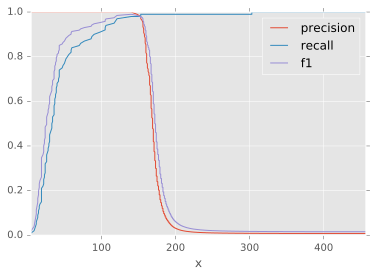
\includegraphics[width=.5\textwidth]{figures/wsj-f1.pdf}
\caption{The precision, recall, and F1 score of codeword detection for $C_c$ being the synthetic WSJ corpus and $C_r$ being the original WSJ corpus}
\label{fig-wsj-f1}
\end{figure}

This experiments represents a highly idealized scenario where

\begin{itemize}
\item I have an exact reference corpus available with the same vocabulary and general language pattern. This is implied by the use of the WSJ corpus as reference corpus (against the synthetic WSJ corpus). A more realistic scenario would be using the Wikipedia corpus or another corpus as the reference corpus against the synthetic WSJ corpus.
\item Codewords are used by the entire population. This is implied by the full substitution process (where every single document in the corpus has codewords substituted).
\item A codeword is never used in another context. For example, if ``cheeseburger'' was a codeword that denotes financial fraud, it is never used to denote the food. This is implied by the substitution process.
\end{itemize}

I can break down these assumptions to see how the embedding + word similarity method performs.

\subsection{Results using Word2Vec on Synthetic WSJ Corpus with External Reference Corpus}

One of the advantages of the word similarity method is that I am not limited by the format of the embeddings. That is, the codeword corpus and the reference corpus do not need to have the same dimensions of embeddings (unlike if I did the original method of cosine matrix rotation). This allows me to use external, pre-trained corpora. Hence, instead of the original WSJ reference corpus, I used Google News and Wikipedia (separately) as reference corpus. Under these (uncleaned and rather different) corpora, the word similarity method performed a lot poorer.

\subsubsection{Google News as Reference Corpus}

I first used the pre-trained Google News corpus available at \url{https://code.google.com/archive/p/word2vec/}. The results were significantly worse than the one using WSJ as the reference corpus.

\begin{figure}[h]
\centering
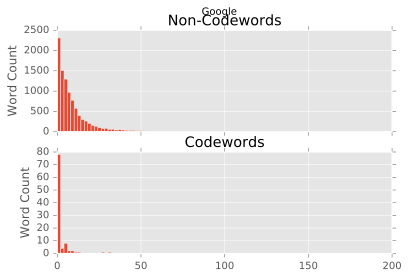
\includegraphics[width=.5\textwidth]{figures/google-count.pdf}
\caption{$x$ for non-codewords and codewords generated for every word $w_{i, c}$ and $w_{i, r}$, with $C_c$ being the synthetic WSJ corpus and $C_r$ being the Google News corpus. Non-codewords and codewords alike have low $x$, even though non-codewords have a higher tail. This results in the high false positive as can be seen in Figure \ref{fig-google-f1}}
\label{fig-google-count}
\end{figure}

\begin{figure}[h]
\centering
\includegraphics[width=.5\textwidth]{figures/google-f1.pdf}
\caption{The precision, recall, and F1 score of codeword detection for $C_c$ being the synthetic WSJ corpus and $C_r$ being the Google News corpus.}
\label{fig-google-f1}
\end{figure}

I observed a high false positive rate. Non-codewords and codewords alike have low $x$, even though non-codewords have a higher tail. This results in the high false positive as can be seen in Figure \ref{fig-google-f1}.

\subsubsection{Wikipedia as Reference Corpus}

I also used the Wikipedia word2vec corpus available at \url{http://textminingonline.com/training-word2vec-model-on-english-wikipedia-by-gensim}. The results were again significantly worse.

\begin{figure}[h]
\centering
\includegraphics[width=.5\textwidth]{figures/wiki-count.pdf}
\caption{$x$ for non-codewords and codewords generated for every word $w_{i, c}$ and $w_{i, r}$, with $C_c$ being the synthetic WSJ corpus and $C_r$ being the Wikipedia corpus. Non-codewords and codewords alike have low $x$, even though non-codewords have a higher tail. This results in the high false positive as can be seen in Figure \ref{fig-wiki-f1}}
\label{fig-wiki-count}
\end{figure}

\begin{figure}[h]
\centering
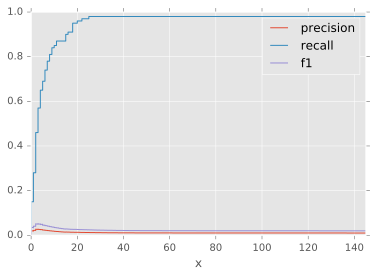
\includegraphics[width=.5\textwidth]{figures/wiki-f1.pdf}
\caption{The precision, recall, and F1 score of codeword detection for $C_c$ being the synthetic WSJ corpus and $C_r$ being the Wikipedia corpus.}
\label{fig-wiki-f1}
\end{figure}

I again observed a high false positive rate. Non-codewords and codewords alike have low $x$, even though non-codewords have a higher tail. This results in the high false positive as can be seen in Figure \ref{fig-wiki-f1}.

This shows that simply using a random external corpus, while intuitively correct, does not produce sufficiently good results due to a large amount of noise. Hence, the choice of reference corpus matters significantly in producing good results.

\subsection{Results using Word2Vec on Synthetic Reddit Corpus with Reddit Reference Corpus}

Next, I test the robustness of this algorithm against the second definition codewords -- that only a small subset of the population (a community) uses the codeword.

\subsubsection{Entire Reddit Corpus}

First, I run an experiment using the easy synthetic Reddit codeword corpus. This is the one with all instances of codewords substituted in the entire corpus (in all 7 communities). In other words, I am simply using a noisier corpus (Reddit) instead of WSJ. This is compared against the original Reddit reference corpus.

\begin{figure}[h]
\centering
\includegraphics[width=.5\textwidth]{figures/reddit-count.pdf}
\caption{$x$ for non-codewords and codewords generated for every word $w_{i, c}$ and $w_{i, r}$, with $C_c$ being the synthetic Reddit corpus and $C_r$ being the original Reddit corpus. Codewords have significantly lower $x$ than non-codewords. However, the standard deviation of the non-codeword distribution is much fatter, resulting in a higher false positive rate as shown in Figure \ref{fig-reddit-f1}}
\label{fig-reddit-count}
\end{figure}

\begin{figure}[h]
\centering
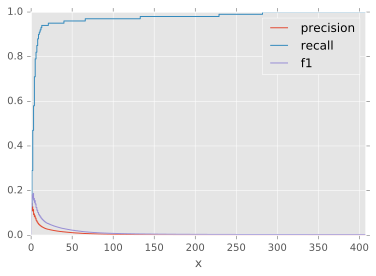
\includegraphics[width=.5\textwidth]{figures/reddit-f1.pdf}
\caption{The precision, recall, and F1 score of codeword detection for $C_c$ being the synthetic Reddit corpus and $C_r$ being the original Reddit corpus.}
\label{fig-reddit-f1}
\end{figure}

I find that performance degrades. Codewords have significantly lower $x$ than non-codewords. However, the standard deviation of the non-codeword distribution is much fatter, resulting in a higher false positive rate as shown in Figure \ref{fig-reddit-f1}. However, we are still able to recall around 80\% of codewords while maintaining a rather low precision and F1 score. This can be attributed to the noise of the Reddit corpus.

\subsubsection{Introducing Communities}

To simulate communities, only 1 of the 7 communities in each of the 7 hard reddit synthetic corpora have substitutions. In other words, for the corpus where the ``humor'' community is defined to have codewords, codeword substitutions are only performed within the portion of the corpus belonging to the ``humor'' metareddit. For example, if the ``hello'' to ``cheeseburger'' substitution is performed, it will only be performed within the ``humor'' community. All the others (``entertainment'', ``gaming'', ``learning'', ``lifestyle'', ``news'', ``television'') do not contain the substitutions.

As shown in Figure \ref{fig-reddit-community-count} and \ref{fig-reddit-community-f1}, the embedding + word similarity method performed significantly worse. There was almost no distinction between codewords and non-codewords.

One reason may be that the Reddit corpus is noisier. However, as I have shown in the earlier experiment involving the \textbf{entire} Reddit corpus, the results from a noisy corpus is still somewhat decent. The more important reason is that of the embedding method I used. Word2Vec assigns a single embedding to each word $i$: $w_{i, r}$ or $w_{i, c}$ in codeword corpus or the reference corpus accordingly. In doing so, this usage assumes that all codewords (e.g. all instances of ``cheeseburger'') are used only in the context of the codeword and not in the original sense. However, if there were \textbf{both} people using ``cheeseburger'' in the sense of the food, and in its codeword context as a fraudulent activity, then a single embedding cannot capture these two different senses. Instead, the embedding would be an average of the two, making no sense whatsoever.

\begin{figure}[H]
\begin{subfigure}[t]{.4\textwidth}
\centering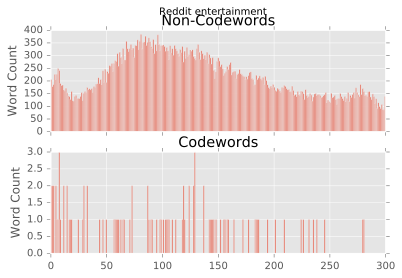
\includegraphics[]{figures/reddit-entertainment-count.pdf}
\caption{``entertainment''}
\label{fig-reddit-entertainment-count}
\end{subfigure}
\begin{subfigure}[t]{.4\textwidth}
\centering\includegraphics[]{figures/reddit-gaming-count.pdf}
\caption{``gaming''}
\label{fig-reddit-gaming-count}
\end{subfigure}
\begin{subfigure}[t]{.4\textwidth}
\centering\includegraphics[]{figures/reddit-humor-count.pdf}
\caption{``humor''}
\label{fig-reddit-humor-count}
\end{subfigure}
\begin{subfigure}[t]{.4\textwidth}
\centering\includegraphics[]{figures/reddit-learning-count.pdf}
\caption{``learning''}
\label{fig-reddit-learning-count}
\end{subfigure}
\begin{subfigure}[t]{.4\textwidth}
\centering\includegraphics[]{figures/reddit-lifestyle-count.pdf}
\caption{``lifestyle''}
\label{fig-reddit-lifestyle-count}
\end{subfigure}
\begin{subfigure}[t]{.4\textwidth}
\centering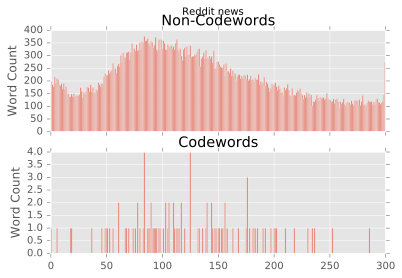
\includegraphics[]{figures/reddit-news-count.pdf}
\caption{``news''}
\label{fig-reddit-news-count}
\end{subfigure}
\begin{subfigure}[t]{.4\textwidth}
\centering\includegraphics[]{figures/reddit-television-count.pdf}
\caption{``television''}
\label{fig-reddit-television-count}
\end{subfigure}
\caption{$x$ for non-codewords and codewords generated for every word $w_{i, c}$ and $w_{i, r}$, with $C_c$ being the hard synthetic Reddit corpus (codewords only in one of the communities) and $C_r$ being the original Reddit corpus.}
\label{fig-reddit-community-count}
\end{figure}

\begin{figure}[H]
\begin{subfigure}[t]{.4\textwidth}
\centering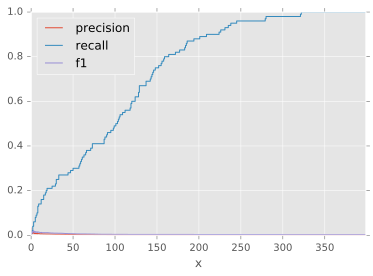
\includegraphics[]{figures/reddit-entertainment-f1.pdf}
\caption{``entertainment''}
\label{fig-reddit-entertainment-f1}
\end{subfigure}
\begin{subfigure}[t]{.4\textwidth}
\centering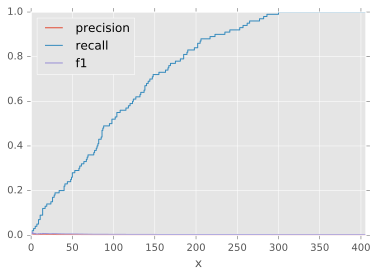
\includegraphics[]{figures/reddit-gaming-f1.pdf}
\caption{``gaming''}
\label{fig-reddit-gaming-f1}
\end{subfigure}
\begin{subfigure}[t]{.4\textwidth}
\centering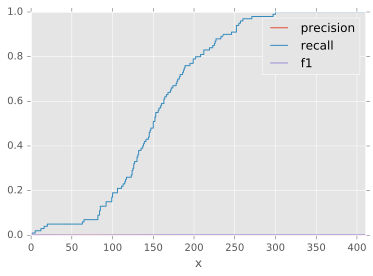
\includegraphics[]{figures/reddit-humor-f1.pdf}
\caption{``humor''}
\label{fig-reddit-humor-f1}
\end{subfigure}
\begin{subfigure}[t]{.4\textwidth}
\centering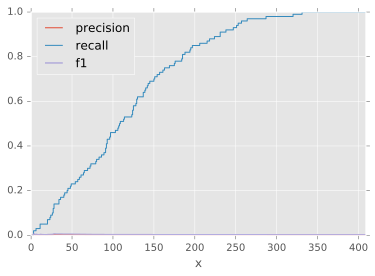
\includegraphics[]{figures/reddit-learning-f1.pdf}
\caption{``learning''}
\label{fig-reddit-learning-f1}
\end{subfigure}
\begin{subfigure}[t]{.4\textwidth}
\centering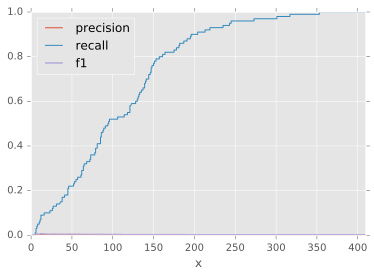
\includegraphics[]{figures/reddit-lifestyle-f1.pdf}
\caption{``lifestyle''}
\label{fig-reddit-lifestyle-f1}
\end{subfigure}
\begin{subfigure}[t]{.4\textwidth}
\centering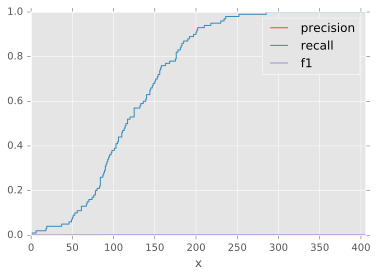
\includegraphics[]{figures/reddit-news-f1.pdf}
\caption{``news''}
\label{fig-reddit-news-f1}
\end{subfigure}
\begin{subfigure}[t]{.4\textwidth}
\centering\includegraphics[]{figures/reddit-television-f1.pdf}
\caption{``television''}
\label{fig-reddit-television-f1}
\end{subfigure}
\caption{The precision, recall, and F1 score of codeword detection for $C_c$ being the hard synthetic Reddit corpus for each of the communities and $C_r$ being the original Reddit corpus.}
\label{fig-reddit-community-f1}
\end{figure}

\newpage

\subsubsection{Verifying the Community Effect}

To further verify that this is indeed the root cause (and not an idiosyncratic effect of the communities in and of themselves) I ran 7 more experiments. Each time, the codeword corpus is \textbf{the substituted subset of the original Reddit corpus belonging to the community} and the reference corpus is \textbf{the subset of the original Reddit corpus belonging to the community}. For example, for the ``humor'' experiment, I will substitute words only within the ``humor'' community, then run Word2Vec on only the ``humor'' community to produce the codeword embeddings. Then, I will take the original corpus from only the ``humor'' community, then run Word2Vec on the original ``humor'' community to produce reference embeddings. In other words, I am isolate each of the individual communities. If there was an idiosyncratic effect on a community level, this should produce bad results. However, if the bad results in the previous section were really the effect of codeword communities existing within a larger population, then the results for this section should be good.

As shown in Figures \ref{fig-reddit-community-only-count} and \ref{fig-reddit-community-only-f1}, the experiments consistently scored highly. The codewords were detected consistently. Hence, I conclude that it is the only the existence of communities that use a word within a codeword context existing within a population that uses the same word in the normal context that causes the problems in the previous experiment.

\begin{figure}[H]
\begin{subfigure}[t]{.4\textwidth}
\centering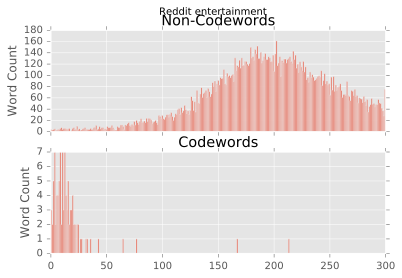
\includegraphics[]{figures/reddit-entertainment-only-count.pdf}
\caption{``entertainment'' only}
\label{fig-reddit-entertainment-only-count}
\end{subfigure}
\begin{subfigure}[t]{.4\textwidth}
\centering\includegraphics[]{figures/reddit-gaming-only-count.pdf}
\caption{``gaming'' only}
\label{fig-reddit-gaming-only-count}
\end{subfigure}
\begin{subfigure}[t]{.4\textwidth}
\centering\includegraphics[]{figures/reddit-humor-only-count.pdf}
\caption{``humor'' only}
\label{fig-reddit-humor-only-count}
\end{subfigure}
\begin{subfigure}[t]{.4\textwidth}
\centering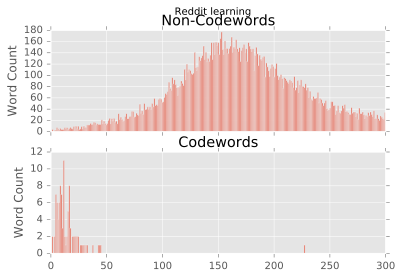
\includegraphics[]{figures/reddit-learning-only-count.pdf}
\caption{``learning'' only}
\label{fig-reddit-learning-only-count}
\end{subfigure}
\begin{subfigure}[t]{.4\textwidth}
\centering\includegraphics[]{figures/reddit-lifestyle-only-count.pdf}
\caption{``lifestyle'' only}
\label{fig-reddit-lifestyle-only-count}
\end{subfigure}
\begin{subfigure}[t]{.4\textwidth}
\centering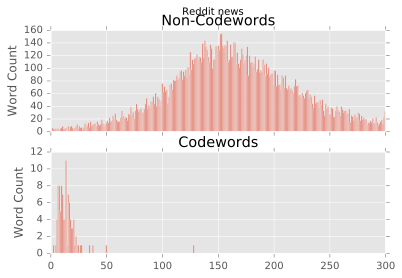
\includegraphics[]{figures/reddit-news-only-count.pdf}
\caption{``news'' only}
\label{fig-reddit-news-only-count}
\end{subfigure}
\begin{subfigure}[t]{.4\textwidth}
\centering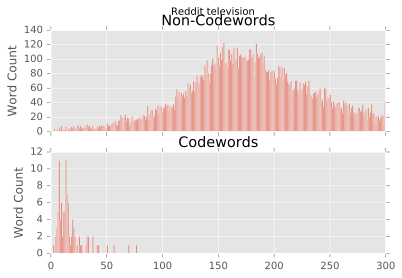
\includegraphics[]{figures/reddit-television-only-count.pdf}
\caption{``television'' only}
\label{fig-reddit-television-only-count}
\end{subfigure}
\caption{$x$ for non-codewords and codewords generated for every word $w_{i, c}$ and $w_{i, r}$, with $C_c$ being the subset of the synthetic Reddit corpus (codewords only the communities) and $C_r$ being the original Reddit corpus.}
\label{fig-reddit-community-only-count}
\end{figure}

\begin{figure}[H]
\begin{subfigure}[t]{.4\textwidth}
\centering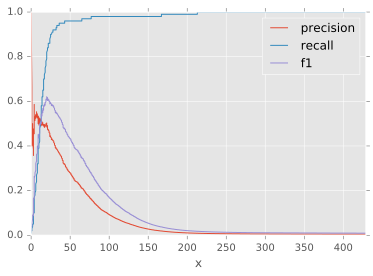
\includegraphics[]{figures/reddit-entertainment-only-f1.pdf}
\caption{``entertainment'' only}
\label{fig-reddit-entertainment-only-f1}
\end{subfigure}
\begin{subfigure}[t]{.4\textwidth}
\centering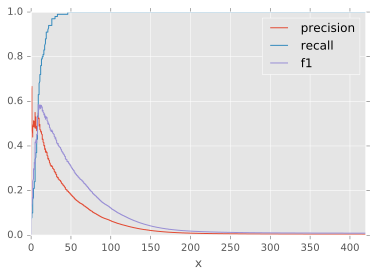
\includegraphics[]{figures/reddit-gaming-only-f1.pdf}
\caption{``gaming'' only}
\label{fig-reddit-gaming-only-f1}
\end{subfigure}
\begin{subfigure}[t]{.4\textwidth}
\centering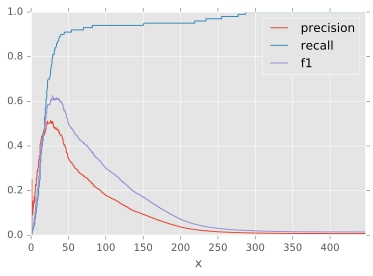
\includegraphics[]{figures/reddit-humor-only-f1.pdf}
\caption{``humor'' only}
\label{fig-reddit-humor-only-f1}
\end{subfigure}
\begin{subfigure}[t]{.4\textwidth}
\centering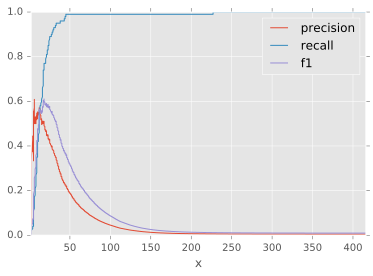
\includegraphics[]{figures/reddit-learning-only-f1.pdf}
\caption{``learning'' only}
\label{fig-reddit-learning-only-f1}
\end{subfigure}
\begin{subfigure}[t]{.4\textwidth}
\centering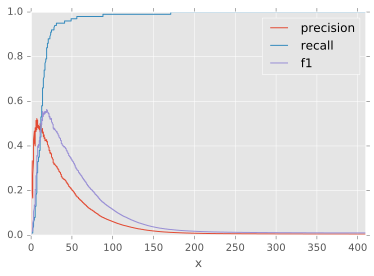
\includegraphics[]{figures/reddit-lifestyle-only-f1.pdf}
\caption{``lifestyle'' only}
\label{fig-reddit-lifestyle-only-f1}
\end{subfigure}
\begin{subfigure}[t]{.4\textwidth}
\centering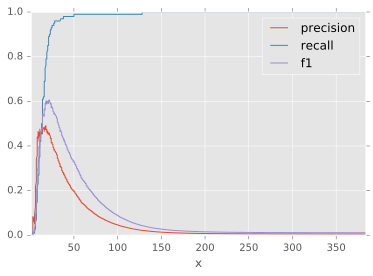
\includegraphics[]{figures/reddit-news-only-f1.pdf}
\caption{``news'' only}
\label{fig-reddit-news-only-f1}
\end{subfigure}
\begin{subfigure}[t]{.4\textwidth}
\centering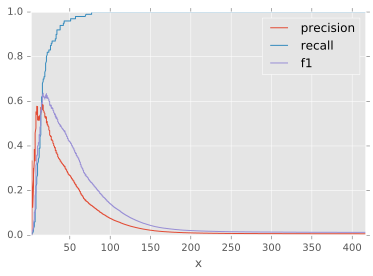
\includegraphics[]{figures/reddit-television-only-f1.pdf}
\caption{``television'' only}
\label{fig-reddit-television-only-f1}
\end{subfigure}
\caption{The precision, recall, and F1 score of codeword detection for $C_c$ being the subset of the synthetic Reddit corpus for each of the communities and $C_r$ being the original Reddit corpus.}
\label{fig-reddit-community-only-f1}
\end{figure}